\section{Tia Nur Candida (1174086)}
\subsection{Menulis Shapefile dengan PySHP}
\begin{enumerate}
	\item Nomor 1
	\lstinputlisting{src/tugas2/1174086/1.py}
	\begin{figure}[H]
		
\includegraphics[width=6cm]{figures/Tugas2/1174086/No1.jpg}
		\centering
		\caption{Point (Titik)}
	\end{figure}
	\item Nomor 2
	\lstinputlisting{src/tugas2/1174086/2.py}
	\begin{figure}[H]
		
\includegraphics[width=6cm]{figures/Tugas2/1174086/No2.jpg}
		\centering
		\caption{Point (Titik)}
	\end{figure}
	\item Nomor 3
	\lstinputlisting{src/tugas2/1174086/3..py}
	\begin{figure}[H]
		
\includegraphics[width=6cm]{figures/Tugas2/1174086/No3.jpg}
		\centering
		\caption{Point (Titik)}
	\end{figure}
	\item Nomor 4
	\lstinputlisting{src/tugas2/1174086/4.py}
	\begin{figure}[H]
		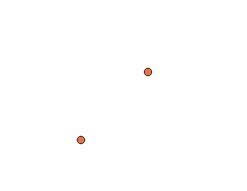
\includegraphics[width=6cm]{figures/Tugas2/1174086/No4.jpg}
		\centering
		\caption{Point (Titik)}
	\end{figure}
	\item Nomor 5
	\lstinputlisting{src/tugas2/1174086/5.py}
	\begin{figure}[H]
		
\includegraphics[width=6cm]{figures/Tugas2/1174086/No5.jpg}
		\centering
		\caption{PolyLine (Garis)}
	\end{figure}
	\item Nomor 6
	\lstinputlisting{src/tugas2/1174086/6.py}
	\begin{figure}[H]
		
\includegraphics[width=6cm]{figures/Tugas2/1174086/No6.jpg}
		\centering
		\caption{Polygon (Bidang)}
	\end{figure}
	\item Nomor 7
	\lstinputlisting{src/tugas2/1174086/7.py}
	\begin{figure}[H]
		
\includegraphics[width=6cm]{figures/Tugas2/1174086/No7.jpg}
		\centering
		\caption{Polygon (Bidang)}
	\end{figure}
	\item Nomor 8
	\lstinputlisting{src/tugas2/1174086/8.py}
	\begin{figure}[H]
		
\includegraphics[width=6cm]{figures/Tugas2/1174086/No8.jpg}
		\centering
		\caption{Polygon (Bidang)}
	\end{figure}
	\item Nomor 9
	\lstinputlisting{src/tugas2/1174086/9.py}
	\begin{figure}[H]
		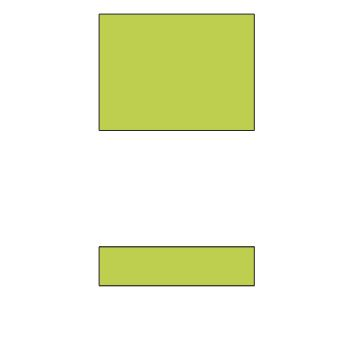
\includegraphics[width=6cm]{figures/Tugas2/1174086/No9.jpg}
		\centering
		\caption{Polygon (Bidang)}
	\end{figure}
	\item Nomor 10
	\lstinputlisting{src/tugas2/1174086/10.py}
	\begin{figure}[H]
		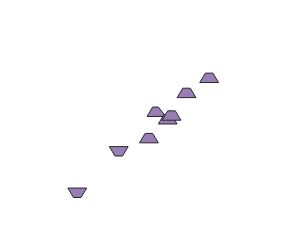
\includegraphics[width=6cm]{figures/Tugas2/1174086/No10.jpg}
		\centering
		\caption{Polygon, Hasil modulus dari npm saya 1174086 adalah 6 jadi membuat bidang trapesium dan angka kedua akhir dari npm saya adalah 8 jadi membuat bidangnya sebanyak 8}
	\end{figure}
\end{enumerate}
\subsection{Link}
https://youtu.be/Kwh-8fr2MRw
